\documentclass[../psets.tex]{subfiles}

\pagestyle{main}
\renewcommand{\leftmark}{Problem Set \thesection}
\stepcounter{section}

\begin{document}




\section{Cycles, Cubes, and the Dodecahedron}
\begin{enumerate}
    \item \marginnote{10/10:}If $\sigma$ is an element of $S_n$, then $\sigma$ has a cycle decomposition into disjoint cycles of various lengths (let us include 1-cycles). Since disjoint cycles commute, the shape of the element is determined by the lengths of the various cycles, which we can assume are put in decreasing order. Any two elements with the same cycle shape are conjugate, so the conjugacy classes are determined by writing $n$ ($=52$, say) as a sum of decreasing integers.
    \begin{enumerate}
        \item Find the conjugacy class in $S_{52}$ with the largest number of elements.
        \begin{proof}
            % Let $52=\sum_{i=1}^ka_i$, where $a_1,\dots,a_k$ is a decreasing set of natural numbers. We begin with a couple of statements and justifications.\par\smallskip
            % There are $(a_i-1)!$ cycles of length $a_i$: There are $a_i!$ permutations of $a_i$ numbers, but for each permutation $(b_1,\dots,b_{a_i})$, there are $a_i$ permutations describing the same cycle, e.g.,
            % \begin{align*}
            %     (b_{a_i},b_1,b_2,\dots,b_{a_i-1})&&
            %     (b_{a_i-1},b_{a_i},b_1,b_2,\dots,b_{a_i-2})
            % \end{align*}
            % so there are $a_i!/a_i=(a_i-1)!$ cycles of length $a_i$ all told.\par
            % The total number of elements in the conjugacy class $\sum_{i=1}^ka_i$ is $\prod_{i=1}^k(a_i-1)!$: We induct on $k$. For the base case $k=1$, there is only one cycle, so naturally the total number of elements is $\prod_{i=1}^1(a_i-1)!=(a_i-1)!$. Now suppose inductively we have proven that the total number of elements in the conjugacy class $\sum_{i=1}^ka_i$ is $\prod_{i=1}^k(a_i-1)!$; we seek to prove the claim for $k+1$. We know that to each product of length $k$ of cycles, there correspond $(a_{k+1}-1)!$ products of length $k-1$ of cycles. In other words, to each of the $\prod_{i=1}^k(a_i-1)!$ products of length $k$ of cycles, there correspond $(a_{k+1}-1)!$ products of length $k-1$ of cycles, so the total number of elements in the conjugacy class is
            % \begin{equation*}
            %     \prod_{i=1}^k(a_i-1)!\cdot(a_{k+1}-1)! = \prod_{i=1}^{k+1}(a_i-1)!
            % \end{equation*}
            % as desired.\par\smallskip
            % The problem now becomes one of finding $\sum_{i=1}^ka_i=52$ such that $\prod_{i=1}^k(a_i-1)!$ is as large as possible. Consider $a_i\geq a_j$. Will it make the product larger or smaller if we redefine $a_i:=a_i+1$ and $a_j:=a_j-1$? This is equivalent to changing the terms in the product from $(a_i-1)!(a_j-1)!$ to $a_i!(a_j-2)!$; indeed, the difference between these two terms is that one smaller $(a_j-1)$ term has been removed, and the larger $a_i$ term has been added in its place. Thus, it is beneficial to, as many times as possible, funnel the numerical value of smaller $a_j$ into larger $a_i$. Note that if $a_j-1=0$, we remove $a_j$ from the sum and decrease $k$ by 1.\par
            % The limit of this process is when we have combined all $a_j$'s of lower value into higher $a_i$'s, ultimately leading to one single $a_1=52$. Therefore, the conjugacy class in $S_{52}$ with the largest number of elements is:
            % \begin{equation*}
            %     \boxed{\text{The conjugacy class containing cycles of length 52.}}
            % \end{equation*}

            Let $52=\sum_{i=1}^kc_ip_i$, where $p_1,\dots,p_k$ is a decreasing sequence of natural numbers describing the cycle lengths present in the conjugacy class and the $c_i\in\N$ are their multiplicities.\par\smallskip
            There are $52!$ permutations of the numbers $1,\dots,52$. We can partition every permutation up into $p_i$-cycles, but in doing so, we will realize that we have overcounted in two ways.\par
            First off, every $p_i$-cycle can be written in $p_i$ equivalent ways. Thus, for every permutation $a_1,\dots,a_{52}$, there are $p_i$ permutations written differently that mean the same thing, so we need to divide through by $p_i$. Doing this for all $p_i$ (and counting multiplicities), we need to divide through by $\prod_{i=1}^kp_i^{c_i}$.\par
            Additionally, disjoint cycles commute. This means that the order in which we write the $c_i$ $p_i$-cycles doesn't matter. Since there are $c_i!$ orders in which we can write the $c_i$ $p_i$-cycles, we also need to divide through by $\prod_{i=1}^kc_i!$.\par
            Therefore, the total number of elements in the conjugacy class $\sum_{i=1}^kc_ip_i$ is
            \begin{equation*}
                \frac{n!}{\prod_{i=1}^kp_i^{c_i}\cdot c_i!}
            \end{equation*}
            This is the functional whose value we want to maximize.\par\smallskip
            To maximize the above functional, we can seek to minimize its denominator. To do so, we'll justify a couple of rules.\par
            First, note that if $p,c\geq 2$, then
            \begin{equation*}
                p^c\cdot c! > cp\cdot 1!
            \end{equation*}
            We can prove this by inducting on $p$ and $c$ in turn, keeping the other fixed. This rule tells us that if we want to minimize the above functional, it is to our benefit to reduce all multiplicities to 1 by combining cycles of the same length (as long as that length is greater than 1).\par
            We are now down to only classes of the form $\sum_{i=1}^kx_i=\sum_{i=1}^kc_ip_i$. Thus, the problem becomes one of minimizing one of the two equations below, depending on whether or not $p_k=1$ (remember that $p_1,\dots,p_k$ is \emph{decreasing}, so 1, if present, will be $p_k$).
            \begin{align*}
                \prod_{i=1}^kc_ip_i &= \prod_{i=1}^kx_i&
                \prod_{i=1}^{k-1}c_ip_i\cdot 1^{c_k}c_k! &= c_k!\prod_{i=1}^{k-1}x_i
            \end{align*}
            With respect to this kind of product, we can note that if $a,b\geq 2$, then
            \begin{equation*}
                ab \geq a+b
            \end{equation*}
            Thus, it is to our benefit to combine all cycles of length greater than 1. Thus, we have reduced to the cases
            \begin{align*}
                52&&
                c_k!(52-c_k)
            \end{align*}
            respectively from the above. Since the right equation above is minimized for $c_k=1$ and, with this value, evaluates to $51<52$, we know that the conjugacy class in $S_{52}$ with the largest number of elements is:
            \begin{equation*}
                \boxed{\text{The conjugacy class }52=51+1.}
            \end{equation*}
        \end{proof}
        \item Find the conjugacy class in $S_{52}$ which contains the element of largest order. (This question is somewhat computational, so an explanation of your strategy plus the answer is sufficient.)
        \begin{proof}
            % Relatively prime? Least common multiple?

            % Optimize $p_1^{v_1}\times\cdots\times p_n^{v_n}$ subject to $\sum p_iv_i\leq 52$ and $p_i,p_j$ are pairwise distinct. Make some more observations: Reduce the number of possibilities you need to consider. Create rules on what $p_1,\dots,p_n$ and $v_1,\dots,v_n$ could be. WLOG, let $p_1<\cdots<p_n$. One possible rule: $v_i=1$, 47 is the biggest prime we can choose. The name of the game: Find rules that reduce the number of cases and then check the cases.
            % Additionally, the way to increase the lcm of a set of numbers as fast as possible while using as small of numbers as possible is to pick the $a_i$ to be primes.\par
            % The problem now becomes one of finding $\sum_{i=1}^ka_i\leq 52$ such that each $a_i$ is prime and $\prod_{i=1}^ka_i$ is as large as possible; any nonzero remainder $52-\sum_{i=1}^ka_i$ can be added in as an additional number that will not augment the lcm but will bring the total up to 52. Casework can confirm that
            % \begin{empheq}[box=\fbox]{align*}
            %     a_1 &= 17&
            %     a_2 &= 13&
            %     a_3 &= 11&
            %     a_4 &= 5&
            %     a_5 &= 3&
            %     a_6 &= 2&
            %     a_7 &= 1
            % \end{empheq}
            % are our desired numbers.

            % 1 should not be a number.

            % All numbers should be distinct.

            % All numbers should be mutually relatively prime.

            % Multiple smaller relatively prime numbers contribute more than a big prime number?
            % Increasing the power of a smaller number helps more than adding a bigger number?
            % Split a big number into smaller relatively prime numbers.

            % Solve the problem with a first guess and then progressive refinement.
            % In the final solution, the lcm of every $n$ in the list with the rest of the list is greater than or equal to the lcm of $m(n-m)$ times the list for all natural numbers $m<n/2$.
            % Suppose $a_1,\dots,a_k$ is the final list. Then
            % \begin{equation*}
            %     \lcm(a_1,\dots,a_k) \geq \lcm(a_1,\dots,a_{i-1},n(a_i-n),a_{i+1},\dots,a_k)
            % \end{equation*}
            % for all $n<a_i$ and all $i$.

            Let $52=\sum_{i=1}^ka_i$. By Exercise 1.3.15 of \textcite{bib:DummitFoote} (and from class), the order of an element of $S_n$ equals the least common multiple (lcm) of the lengths of the cycles in its cycle decomposition. Thus, all elements in a conjugacy class have the same order.\par
            We now must optimize $\lcm(a_1,\dots,a_k)$ over all such decompositions. To do so, we will start with a guess based on some observations and then progressively refine according to two rules.\par
            Observations:
            \begin{enumerate}[label={(\arabic*)}]
                \item Rely (primarily) on relatively prime numbers. For example, the list $2,4,8$ has $\lcm=8$, but the list $2,3,5$ has $\lcm=30$, and a smaller sum.
                \item 1 should not be in the list because it does not contribute anything to the lcm but does add to the sum.
                \item Rely (primarily) on small numbers --- remember the $ab\geq a+b$ rule for $a,b\geq 2$ from part (a). This means that it is often beneficial to split larger numbers into smaller numbers.
            \end{enumerate}
            With these observations in hand, we'll use as our starting list
            \begin{equation*}
                2,3,5,7,11,13,11
            \end{equation*}
            where we include the last 11 because $2+\cdots+13=41$ and $52-41=11$, i.e., we cannot include the first six numbers and the next prime (17) without the sum exceeding 52.\par\smallskip
            We now give the two rules for progressive refinement of the above list. The first one is that if $a_1,\dots,a_k$ is the final list, then
            \begin{equation*}
                \lcm(a_1,\dots,a_k) \geq \lcm(a_1,\dots,a_{i-1},n,(a_i-n),a_{i+1},\dots,a_k)
            \end{equation*}
            for all $n<a_i$ and all $i\leq k$. The second one is that if $a_1,\dots,a_k$ is the final list, then
            \begin{equation*}
                \lcm(a_1,\dots,a_k) \geq \lcm(a_1,\dots,a_{i-1},a_{i+1},\dots,a_{j-1},a_{j+1},\dots,a_k,a_i+a_j)
            \end{equation*}
            for all $i\neq j\leq k$. In particular, if we ever come across a case in which either of the above two inequalities is not satisfied, then we should redefine our list on the LHS with the list on the RHS.\par
            Using these rules, we will first attack the second 11 in the above list. We can compute that
            \begin{equation*}
                \lcm(2,3,5,7,11,13,11) = 30030
            \end{equation*}
            and that
            \begin{equation*}
                \lcm(2,3,5,7,11,13,1,10) = 30030
            \end{equation*}
            but that
            \begin{equation*}
                \lcm(2,3,5,7,11,13,2,9) = 90090
            \end{equation*}
            Thus, we redefine our list to be $2,2,3,5,7,9,11,13$. If we run through and check all of the cases by the first rule, we will find that there is no more splitting we can do to increase the value of this list. However, by the second rule, there is some combining: If we combine $2,2\mapsto 4$, then
            \begin{equation*}
                \lcm(3,4,5,7,9,11,13) = 180180
            \end{equation*}
            Running both rules, we will find that we cannot progressively refine any further from here. Therefore, the conjugacy class in $S_{52}$ which contains the element of the largest order is:
            \begin{equation*}
                \boxed{\text{The conjugacy class }52 = 13+11+9+7+5+4+3.}
            \end{equation*}
        \end{proof}
    \end{enumerate}
    \item Let $k\leq n$ be even. Prove that every element in $S_n$ can be written as a product of $k$-cycles.
    \begin{proof}
        % Let
        % \begin{equation*}
        %     (a_1,\dots,a_{m_1})(a_{m_1+1},\dots,a_{m_2})\cdots(a_{m_{i-1}+1},\dots,a_{m_i})
        % \end{equation*}
        % where $m_i=n$ be an arbitrary element of $S_n$.

        % Something with transpositions. A transposition is a 2-cycle and every element in $S_n$ can be written as a product of transpositions. That's where the even comes in. But how do I generalize a transposition to a 4-cycle? A 6-cycle? A $2n$-cycle? We can also go to adjacent transpositions. Disjoint transpositions commute.

        Every element in $S_n$ can be written in terms of elementary transpositions. Thus, the problem becomes one of showing that every elementary transposition can be written as a product of $k$-cycles.\par
        Let $(i,i+1)\in S_n$ be an elementary transposition. We will prove that
        \begin{equation*}
            \begin{split}
                (i,i+1) ={}& (i,i+_n1,\dots,i+_n(k-1))^2\\
                &\cdot (i,i+_n(k-1),i+_n(k-3),\dots,i+_n3,i+1,i+_n(k-2),i+_n(k-4),\dots,i+_n2)
            \end{split}
        \end{equation*}
        where $+_n$ denotes addition modulo $n$\footnote{Motivation: We have, for example, that $(1,2)\in S_n$ with $k=8$ can be given by $(1,2,3,4,5,6,7,8)^2(1,8,6,4,2,7,5,3)$. Essentially, what we are doing here is sending $1\mapsto 8$ and $2\mapsto 7$ so that when we rotate all of the numbers twice (with $(1,\dots,8)^2$), 1 and 2 land in the 2 and 1 positions. The "decreasing by 2 at a time" part is a necessary consequence of writing an 8-cycle that sends $1\mapsto 8$ and $2\mapsto 7$ and can be more easily understood by drawing out a function diagram and tracing the cycle.}. Indeed, we have that
        \begin{align*}
            \begin{split}
                & (i,i+_n1,\dots,i+_n(k-1))\\
                &\cdot (i,i+_n1,\dots,i+_n(k-1))\\
                &\cdot (i,i+_n(k-1),i+_n(k-3),\dots,i+_n3,i+1,i+_n(k-2),i+_n(k-4),\dots,i+_n2)
            \end{split}\\
            \begin{split}
                ={}& (i,i+_n1,\dots,i+_n(k-1))\\
                &\cdot (i)(i+1,i+_n(k-1),i+_n(k-2),\dots,i+_n2)
            \end{split}\\
            \begin{split}
                ={}& (i,i+_n1,\dots,i+_n(k-1))\\
                &\cdot (i+1,i+_n(k-1),i+_n(k-2),\dots,i+_n2)
            \end{split}\\
            ={}& (i,i+1)
        \end{align*}
        as desired.
    \end{proof}
    \item Let $D$ be a regular dodecahedron. You may assume for this question that it is possible to inscribe a cube $C$ on the vertices of $D$ as shown below.
    \begin{center}
        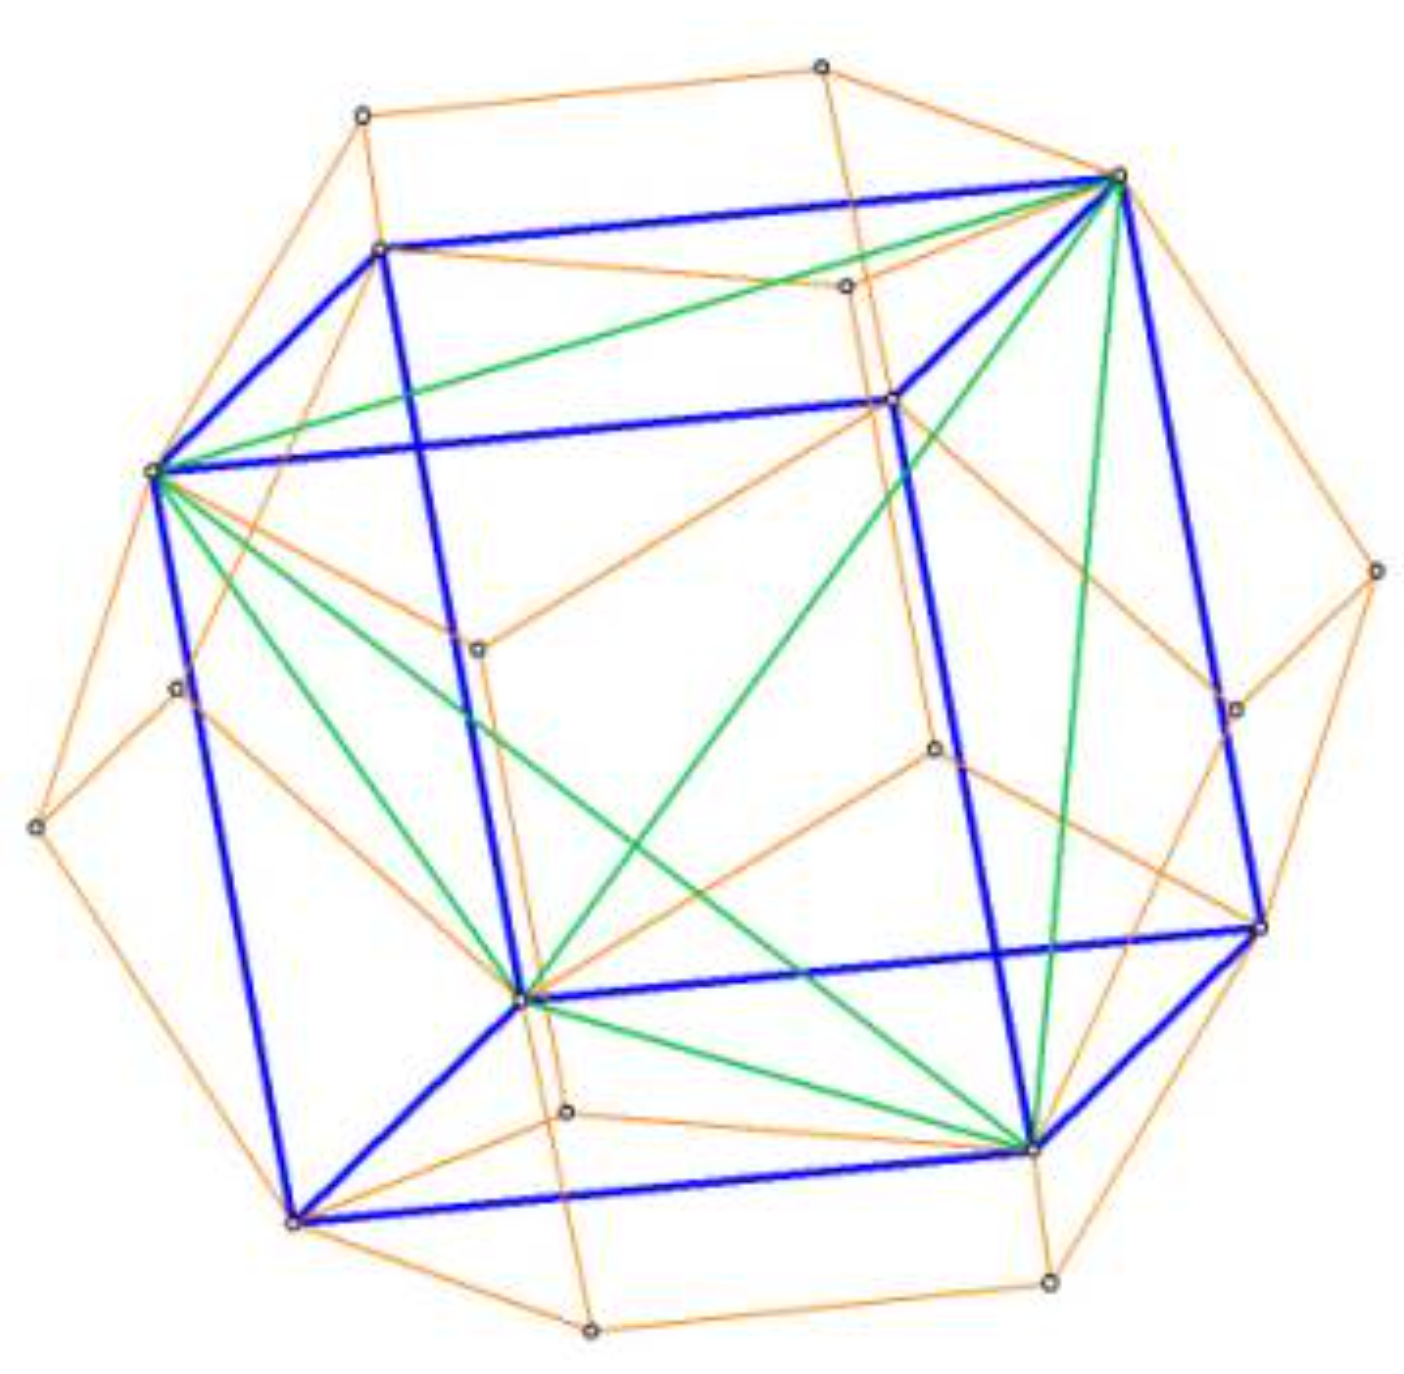
\includegraphics[width=0.4\linewidth]{../ExtFiles/dodecahedronCube.png}
    \end{center}
    \emph{Remember the following distinction}: An object $X$ in $\R^3$ is \textbf{fixed pointwise} by $g$ if every point on $X$ is fixed by $g$, that is, if $gx=x$ for all $x\in X$. An object $X\in\R^3$ is \textbf{preserved} by $g$ if every point on $X$ maps to another (possibly different) point on $X$, i.e., for all $x\in X$, there exists $y\in X$ such that $gx=y$. As an example, the circle centered at the origin is preserved by any rotation through the origin, but is not fixed pointwise unless the rotation is trivial.
    \begin{itemize}
        \item If $F$ is a face, call a line between two vertices of $F$ an \textbf{internal line} if the vertices are not adjacent. That is, an internal line is a line between two vertices of a pentagonal face which is not an edge of the pentagon.
        \item Observe that the cube $C$ has 12 edges, and that each edge lies on exactly one of the 12 faces of $D$ as an internal line.
        \item Choose a face $F$ of $D$ and let $g$ be the symmetry of $D$ of order 5 which is a rotation by $2\pi/5$ through the line passing through the middle of $F$ and the middle of the opposite face $-F$.
        \item Label the vertices of a face $F$ from 1 to 5. Suppose that $C=C_{(1,3)}$ intersects $F$ in the internal edge from 1 to 3.
    \end{itemize}
    \begin{enumerate}
        \stepcounter{enumii}
        \item Show that for any such $g$, the five cubes $C_{(1,3)}$, $C_{(2,4)}$, $C_{(3,5)}$, $C_{(1,4)}$, and $C_{(2,5)}$ obtained by applying the powers of $g$ to each cube are distinct because they intersect $F$ in different internal lines (which are the lines between vertices indicated by the notation).
        \begin{proof}
            Let $g$ be arbitrary. Choose the $z$-axis to be the axis about which $g$ rotates the dodecahedron/cube. Adopt a cylindrical coordinate system $(r,\theta,z)$. Orient the remaining coordinate axes so that vertex 1 of face $F$ lies at $(r,0,z)$; it follows that vertices 2-5 lie at $(r,2\pi/5,z)$, $(r,4\pi/5,z)$, $(r,6\pi/5,z)$, and $(r,8\pi/5,z)$, respectively. In this coordinate system, $g^n$ is the orthogonal transformation that sends
            \begin{equation*}
                (r,\theta,z) \mapsto \left( r,\theta+\frac{2\pi n}{5},z \right)
            \end{equation*}\par
            Consider $C_{(1,3)}$, which intersects $F$ at the internal line from vertex 1 to vertex 3. Applying the powers of $g$ sends
            \begin{align*}
                g(1) &= g(r,0,z) = (r,2\pi/5,z) = 2&
                    g(3) &= g(r,4\pi/5,z) = (r,6\pi/5,z) = 4\\
                g^2(1) &= g^2(r,0,z) = (r,4\pi/5,z) = 3&
                    g^2(3) &= g^2(r,4\pi/5,z) = (r,8\pi/5,z) = 5\\
                g^3(1) &= g^3(r,0,z) = (r,6\pi/5,z) = 4&
                    g^3(3) &= g^3(r,4\pi/5,z) = (r,2\pi,z) = (r,0,z) = 1\\
                g^4(1) &= g^4(r,0,z) = (r,8\pi/5,z) = 5&
                    g^4(3) &= g^4(r,4\pi/5,z) = (r,2\pi/5,z) = 2\\
                g^5(1) &= e(r,0,z) = 1&
                    g^5(3) &= e(r,4\pi/5,z) = 3
            \end{align*}
            Thus, we know that the cube $g(C_{(1,3)})$ --- remember that $g$, as an orthogonal transformation, preserves lengths, angles, and lines, so the image of a cube under $g$ will still be a cube --- intersects $F$ at the internal line from vertex 2 to vertex 4, the cube $g^2(C_{(1,3)})$ intersects $F$ at the internal line from vertex 3 to vertex 5, the cube $g^3(C_{(1,3)})$ intersects $F$ at the internal line from vertex 4 to vertex 1, the cube $g^4(C_{(1,3)})$ intersects $F$ at the internal line from vertex 5 to vertex 2, and the cube $g^5(C_{(1,3)})=e(C_{(1,3)})=C_{(1,3)}$ since $g$ is of order 5 by definition. Naturally, continuing onto higher natural numbers will just get us back to these same cubes. It follows that these cubes --- which are equal to $C_{(2,4)}$, $C_{(3,5)}$, $C_{(4,1)}=C_{(1,4)}$, $C_{(5,2)}=C_{(2,5)}$, and $C_{(1,3)}$, respectively --- are all distinct because they intersect $F$ in different internal lines.
        \end{proof}
        \item Show that \emph{any} symmetry of $D$ takes $C$ to one of these five cubes. Hint: Any pair of cubes share two vertices $\mathbf{v},\mathbf{w}$ on $F$ lying on an internal line of $F$ which are connected by an edge of the cube. Given a cube centered at the origin with vertices $\mathbf{v},\mathbf{w}$ and $|\mathbf{v}|=|\mathbf{w}|$ connected by an edge, show that the eight vertices of the cube are
        \begin{equation*}
            \pm\mathbf{v},\ \pm\mathbf{w},\ \pm\mathbf{u}\pm\left( \frac{\mathbf{v}-\mathbf{w}}{2} \right)
        \end{equation*}
        where $\mathbf{u}$ is the (unique up to a $\pm$ sign) vector with $3|\mathbf{u}|^2=2|\mathbf{v}|^2=2|\mathbf{w}|^2$ and $\mathbf{u}\cdot\mathbf{v}=\mathbf{u}\cdot\mathbf{w}=0$.
        \begin{proof}
            % Let $C$ be an arbitrary cube inscribed on the vertices of $D$, and let $h$ be an arbitrary symmetry of $D$. As a symmetry, $h$ sends all vertices of $D$, including those in $D\cap C$, to other vertices of $D$. As an orthogonal map, $h$ sends $C$ to some other cube $h(C)$ (not a rectangular prism or parallelepiped or other deformed variant) inscribed in $D$.\par
            % Let $F$ be a face of $D$. By observation 2, both $C$ and $h(C)$ intersect $F$ at some internal line. Suppose $C$ intersects $F$ at the internal line connecting vertices $\mathbf{v}$ and $\mathbf{w}$.


            % The hint tells us that the rest of the vertices of $C$ are determined from the first two. We need to prove that there's no other different inscribed cube which intersects $F$ at the same internal line.

            % We define a \textbf{cube} (centered at the origin) to be any set of 8 points which are orthogonally related to the set

            % considered in part (b). By observation 2, $C$ intersects $F$ at an internal line of $F$; we may number the vertices of $F$ such that $C=C_{(1,3)}$. 

            {\color{white}hi}\par
            \underline{Setup}: Let $C$ be an arbitrary cube inscribed on the vertices of $D$, and let $F$ be a face of $D$. By the second bullet point above, $C$ intersects $F$ at exactly one of its internal lines. Let $\mathbf{v},\mathbf{w}$ be the vertices of $F$ which are connected by said internal line. Define
            \begin{equation*}
                \mathbf{u} = \sqrt{\frac{2}{3}}|\mathbf{v}|\cdot\frac{\mathbf{v}\times\mathbf{w}}{|\mathbf{v}\times\mathbf{w}|}
            \end{equation*}
            By the definition of the cross product, $\mathbf{u}$ is orthogonal to $\mathbf{v},\mathbf{w}$. Additionally, the way it is defined guarantees that it satisfies the magnitude relation.\par\smallskip
            \underline{Proving the hint}: We now prove that the eight vertices of $C$ are
            \begin{equation*}
                \pm\mathbf{v},\ \pm\mathbf{w},\ \pm\mathbf{u}\pm\left( \frac{\mathbf{v}-\mathbf{w}}{2} \right)
            \end{equation*}
            Let $A$ be the determinant 1, orthogonal transformation which sends $\mathbf{v}\mapsto(a,a,a)$ and $\mathbf{w}\mapsto(-a,a,a)$ for some $a\in\R$. We know that such a transformation exists since it is equivalent to redrawing the basis of $\R^3$ such that the three axes go through the center of three adjacent faces of the cube. Since orthogonal transformations preserve the cross product, we know that
            \begin{align*}
                A\mathbf{u} &= \frac{\sqrt{2/3}|\mathbf{v}|}{|\mathbf{v}\times\mathbf{w}|}\cdot A\mathbf{v}\times A\mathbf{w}\\
                &= \frac{\sqrt{2/3}|A\mathbf{v}|}{|A\mathbf{v}\times A\mathbf{w}|}\cdot
                \begin{pmatrix}
                    0\\
                    -2a^2\\
                    2a^2\\
                \end{pmatrix}\\
                &= \frac{\sqrt{2/3}\cdot\sqrt{3a^2}}{\sqrt{8a^4}}\cdot
                \begin{pmatrix}
                    0\\
                    -2a^2\\
                    2a^2\\
                \end{pmatrix}\\
                &= \frac{1}{2a}\cdot
                \begin{pmatrix}
                    0\\
                    -2a^2\\
                    2a^2\\
                \end{pmatrix}\\
                &=
                \begin{pmatrix}
                    0\\
                    -a\\
                    a\\
                \end{pmatrix}
            \end{align*}
            It follows that the full set of vertices of this cube can be expressed in terms of $\mathbf{u},\mathbf{v},\mathbf{w}$ as follows.
            \begin{align*}
                (a,a,a) &= A(\mathbf{v})\\
                (-a,-a,-a) &= A(-\mathbf{v})\\
                (-a,a,a) &= A(\mathbf{w})\\
                (a,-a,-a) &= A(-\mathbf{w})\\
                (a,-a,a) &= (0,-a,a)+\left( \frac{a-(-a)}{2},a-a,a-a \right)
                    = A\left( \mathbf{u}+\frac{\mathbf{v}-\mathbf{w}}{2} \right)\\
                (-a,-a,a) &= A\left( \mathbf{u}-\frac{\mathbf{v}-\mathbf{w}}{2} \right)\\
                (a,a,-a) &= A\left( -\mathbf{u}+\frac{\mathbf{v}-\mathbf{w}}{2} \right)\\
                (-a,a,-a) &= A\left( -\mathbf{u}-\frac{\mathbf{v}-\mathbf{w}}{2} \right)
            \end{align*}
            Thus, the vertices of $C$ are given by the arguments of $A$, above, as desired.\par\smallskip
            \underline{Proving the claim}: To prove that any symmetry of $D$ takes $C$ to one of the five cubes from part (b), we will let $h$ be an arbitrary symmetry of $D$ and prove that $h$ maps the eight vertices of $C$ to the eight vertices of $C_{(1,3)}$, $C_{(2,4)}$, $C_{(3,5)}$, $C_{(1,4)}$, or $C_{(2,5)}$. Per the hint, we know that $\mathbf{v},\mathbf{w}$ uniquely determine the remainder of the vertices of an inscribed cube. In particular, for each of the five cubes just listed, they are the unique cube which intersects $F$ at the internal line that they do. Thus, since $h$ will send $C$ to some other inscribed cube, which must by observation 2 intersect $F$ in one of the above internal lines, we know that $h$ sends $C$ to one of the five desired cubes.
        \end{proof}
        \item Let $\mathbf{v}_i$ indicate the vector corresponding to vertex $i$ of $F$. Deduce that there are exactly two cubes which have $\mathbf{v}_i$ as a vertex, and that the only vertices that these two cubes have in common are $\pm\mathbf{v}_i$.
        \begin{proof}
            % {\color{white}hi}
            % \begin{itemize}
            %     \item Exactly two cubes have $\mathbf{v}_i$ as a vertex.
            %     \begin{itemize}
            %         \item Parts (b-c): There are exactly 5 distinct cubes inscribed in $D$, which are $C_{(1,3)}$, $C_{(2,4)}$, $C_{(3,5)}$, $C_{(1,4)}$, and $C_{(2,5)}$.
            %         \item Each vertex 1-5 appears exactly twice and in exactly two different cubes according to the above list, as desired.
            %     \end{itemize}
            %     \item The only vertices these two cubes have in common are $\pm\mathbf{v}_i$.
            %     \begin{itemize}
            %         \item We will prove this for $\mathbf{v}_1$; the argument is analogous for $\mathbf{v}_2$-$\mathbf{v}_5$.
            %         \item $C_{(1,3)}$ and $C_{(1,4)}$ both have $\mathbf{v}_1$ as a vertex. The two vertices these cubes have on $F$ are $\mathbf{v}_1,\mathbf{v}_3$ and $\mathbf{v}_1,\mathbf{v}_4$, respectively.
            %         \item Part (c): The eight vertices of each cube are
            %         \begin{align*}
            %             \pm\mathbf{v}_1,\ \pm\mathbf{v}_3,\ \pm\mathbf{u}_{13}\pm\left( \frac{\mathbf{v}_1-\mathbf{v}_3}{2} \right)&&
            %             \pm\mathbf{v}_1,\ \pm\mathbf{v}_4,\ \pm\mathbf{u}_{14}\pm\left( \frac{\mathbf{v}_1-\mathbf{v}_4}{2} \right)
            %         \end{align*}
            %         \item Evidently, the only overlap is at $\pm\mathbf{v}_1$ for $\mathbf{v}_3,\mathbf{v}_4$ distinct.
            %     \end{itemize}
            % \end{itemize}


            We will first prove that exactly two cubes have $\mathbf{v}_i$ as a vertex. By parts (b-c), there are exactly 5 distinct cubes inscribed in $D$: $C_{(1,3)}$, $C_{(2,4)}$, $C_{(3,5)}$, $C_{(1,4)}$, and $C_{(2,5)}$. Since each vertex from 1-5 appears exactly twice and in exactly two different cubes according to the above list, we have the desired result for all $i$.\par
            We now prove that two cubes that both have $\mathbf{v}_i$ as a vertex only share $\pm\mathbf{v}_i$. In particular, we will prove the claim for $\mathbf{v}_1$; the argument is analogous for $\mathbf{v}_2$-$\mathbf{v}_5$. Let's begin. We know that $C_{(1,3)}$ and $C_{(1,4)}$ both have $\mathbf{v}_1$ as a vertex. We also know that the two vertices these cubes have on $F$ are $\mathbf{v}_1,\mathbf{v}_3$ and $\mathbf{v}_1,\mathbf{v}_4$, respectively. Thus, we have by part (c) that the eight vertices of the respective cubes are
            \begin{align*}
                \pm\mathbf{v}_1,\ \pm\mathbf{v}_3,\ \pm\mathbf{u}_{13}\pm\left( \frac{\mathbf{v}_1-\mathbf{v}_3}{2} \right)&&
                \pm\mathbf{v}_1,\ \pm\mathbf{v}_4,\ \pm\mathbf{u}_{14}\pm\left( \frac{\mathbf{v}_1-\mathbf{v}_4}{2} \right)
            \end{align*}
            Evidently, the only overlap is at $\pm\mathbf{v}_1$ for $\mathbf{v}_3,\mathbf{v}_4$ distinct, as desired.
        \end{proof}
        \item (*) Show that any rigid motion of $D$ (i.e., any element of $\text{SO}(3)$ preserving $D$) permutes the 5 cubes. Hint: Show that if a symmetry $\sigma$ preserves the two cubes passing through $\mathbf{v}_i$, then it preserves their intersection and deduce that
        \begin{equation*}
            \sigma\mathbf{v}_i = \pm\mathbf{v}_i
        \end{equation*}
        Deduce that this identity must hold for every $i$, and use this (and HW1) to show that this implies that $\sigma$ is the identity.
        \begin{proof}
            % {\color{white}hi}
            % \begin{itemize}
            %     \item Hint:
            %     \begin{itemize}
            %         \item $\sigma$ preserves $C_{(1,3)},C_{(1,4)}$ implies $\sigma$ preserves $C_{(1,3)}\cap C_{(1,4)}$.
            %         \begin{itemize}
            %             \item Let
            %             \begin{align*}
            %                 C_{(1,3)} &= \left\{ \pm\mathbf{v}_1,\ \pm\mathbf{v}_3,\ \pm\mathbf{u}_{13}\pm\left( \frac{\mathbf{v}_1-\mathbf{v}_3}{2} \right) \right\}&
            %                 C_{(1,4)} &= \left\{ \pm\mathbf{v}_1,\ \pm\mathbf{v}_4,\ \pm\mathbf{u}_{14}\pm\left( \frac{\mathbf{v}_1-\mathbf{v}_4}{2} \right)\right\}
            %             \end{align*}
            %             \item $\sigma$ preserves $C_{(1,3)}$ and $C_{(1,4)}$:
            %             \begin{align*}
            %                 \sigma(C_{(1,3)}) &= C_{(1,3)}&
            %                 \sigma(C_{(1,4)}) &= C_{(1,4)}
            %             \end{align*}
            %             \item $\pm\mathbf{v}_1\in C_{(1,3)}$ and $\sigma(C_{(1,3)})=C_{(1,3)}$: $\sigma(\pm\mathbf{v}_1)\in C_{(1,3)}$.
            %             \item $\pm\mathbf{v}_1\in C_{(1,4)}$ and $\sigma(C_{(1,4)})=C_{(1,4)}$: $\sigma(\pm\mathbf{v}_1)\in C_{(1,4)}$.
            %             \item $\sigma(\pm\mathbf{v}_1)\in C_{(1,3)}$ and $\sigma(\pm\mathbf{v}_1)\in C_{(1,4)}$: $\sigma(\pm\mathbf{v}_1)\in C_{(1,3)}\cap C_{(1,4)}$.
            %             \item Part (d): $C_{(1,3)}\cap C_{(1,4)}=\{\pm\mathbf{v}_1\}$.
            %             \item Last 2: $\sigma(C_{(1,3)}\cap C_{(1,4)})=C_{(1,3)}\cap C_{(1,4)}$.
            %         \end{itemize}
            %         \item $\sigma\mathbf{v}_1=\pm\mathbf{v}_1$.
            %         \begin{itemize}
            %             \item $\sigma(C_{(1,3)}\cap C_{(1,4)})=C_{(1,3)}\cap C_{(1,4)}$ and $C_{(1,3)}\cap C_{(1,4)}=\{\pm\mathbf{v}_1\}$: $\sigma(\mathbf{v}_1)\in\{\pm\mathbf{v}_1\}$.
            %             \item The above: $\sigma\mathbf{v}_1=\pm\mathbf{v}_1$.
            %         \end{itemize}
            %         \item The proof for the remaining $i$ is entirely analogous.
            %         \item Suppose (contradiction): $\sigma\mathbf{v}_1=-\mathbf{v}_1$.
            %         \begin{itemize}
            %             \item If $\sigma$ is to do this \emph{and} be a rigid transformation, it must rotate $C_{(1,3)}$ by $\pi$ radians about $\mathbf{v}_3$, and then may additionally rotate it by $2\pi/3$ or $4\pi/3$ radians about $\mathbf{v}_1$. Note that any of these three transformations does preserve $C_{(1,3)}$, as desired.
            %             \item Similarly, since $\sigma$ preserves $C_{(1,4)}$, it must rotate $C_{(1,4)}$ by $\pi$ radians about $\mathbf{v}_4$, and then may additionally rotate it by $2\pi/3$ or $4\pi/3$ radians about $\mathbf{v}_1$.
            %             \item But these transformations are not equal?
            %             \item Rotation by $\pi/2$ about $z$, then $y$, then $x$ for $C_{(3,1)}$.
            %             \begin{equation*}
            %                 \underbrace{
            %                     \begin{pmatrix}
            %                         1 & 0 & 0\\
            %                         0 & 0 & -1\\
            %                         0 & 1 & 0\\
            %                     \end{pmatrix}
            %                 }_x\underbrace{
            %                     \begin{pmatrix}
            %                         0 & 0 & 1\\
            %                         0 & 1 & 0\\
            %                         -1 & 0 & 0\\
            %                     \end{pmatrix}
            %                 }_y\underbrace{
            %                     \begin{pmatrix}
            %                         0 & -1 & 0\\
            %                         1 & 0 & 0\\
            %                         0 & 0 & 1\\
            %                     \end{pmatrix}
            %                 }_z
            %                 =
            %                 \begin{pmatrix}
            %                     0 & 0 & 1\\
            %                     0 & -1 & 0\\
            %                     1 & 0 & 0\\
            %                 \end{pmatrix}
            %             \end{equation*}
            %             \item Rotation by $2\pi/3$ about $(1,1,-1)$. Send $x\mapsto -z$, $-z\mapsto y$, $y\mapsto x$.
            %             \begin{equation*}
            %                 \begin{pmatrix}
            %                     0 & 1 & 0\\
            %                     0 & 0 & -1\\
            %                     -1 & 0 & 0\\
            %                 \end{pmatrix}
            %             \end{equation*}
            %             \item Rotation by $4\pi/3$ about $(1,1,-1)$. Send $x\mapsto -z$, $-z\mapsto y$, $y\mapsto x$.
            %             \begin{equation*}
            %                 \begin{pmatrix}
            %                     0 & 1 & 0\\
            %                     0 & 0 & -1\\
            %                     -1 & 0 & 0\\
            %                 \end{pmatrix}^2
            %                 =
            %                 \begin{pmatrix}
            %                     0 & 0 & -1\\
            %                     1 & 0 & 0\\
            %                     0 & -1 & 0\\
            %                 \end{pmatrix}
            %             \end{equation*}
            %         \end{itemize}
            %     \end{itemize}
            % \end{itemize}


            We will first prove the hint. Let's begin.\par
            Suppose $\sigma$ preserves the two cubes $C,C'$ passing through $\mathbf{v}_i$. To prove that $\sigma$ preserves $C\cap C'$, it will suffice to show that $\sigma$ maps every element in that set to another element of that set. Since $C\cap C'=\{\pm\mathbf{v}_i\}$ by part (d), we confirm this with two cases. For $\mathbf{v}_i$, since $\mathbf{v}_i\in C$ and $\sigma$ preserves $C$, we know that $\sigma\mathbf{v}_i\in C$. Similarly, we know that $\sigma\mathbf{v}_i\in C'$. Thus, by the definition of a set union, $\sigma\mathbf{v}_i\in C\cap C'$, as desired. An analogous argument treats the other case.\par
            It follows from the above that $\sigma\mathbf{v}_i\in\{\pm\mathbf{v}_i\}$. Therefore,
            \begin{equation*}
                \sigma\mathbf{v}_i = \pm\mathbf{v}_i
            \end{equation*}
            as desired.\par
            Now suppose for the sake of contradiction that $\sigma\mathbf{v}_1=-\mathbf{v}_1$. Then for $\sigma$ to be orthogonal, we must necessarily have $\sigma\mathbf{v}_i=-\mathbf{v}_i$ for all $i$. But then $\sigma$ is an inversion with determinant $-1$, and is thus not a rigid motion, a contradiction. Therefore, we must have that $\sigma\mathbf{v}_i=\mathbf{v}_i$ for all $i$. It follows by HW1, Q2f since $\sigma$ fixes (at least) two linearly independent vectors that $\sigma$ is the identity.
        \end{proof}
        \item Deduce that the symmetry group of the dodecahedron is a subgroup of $S_5$ of order 60.
        \begin{proof}
            % Every rigid motion of the dodechedron is a permutation of 5 things (cubes); that's how we get the last part.

            % The point of the question is that you should study $I$ through its "action" on the inscribed cubes.
            % Part (a) is a definition of $C_{(a,b)}$. There's nothing to do; don't write anything.
            % Part (b): Let $S$ denote the set of dodecahedrons with inside cubes. $|S|\geq 5$.
            % Part (c): $|S|=5$.
            % Part (d): Is what it is; pretty straightforward.
            % Part (e): Not only does $G$ map to $S_5$, but it is an injection from $G$ to $S_5$.
            % Part (f): Bringing size 60 into the picture. There's a lower bound; show it's size 60. There should be an upper bound based on sign. $60=12\cdot 5$. Find a 


            By part (f), any rigid motion of $D$ permutes the 5 cubes, and is thus an element of $S_5$. Moreover, said rigid motion must correspond to a positive-determinant matrix element of $\text{SO}(3)$. Thus, since half of $S_5$ maps to $\text{SO}(3)$ and the other half maps to $\text{O}(3)\setminus\text{SO}(3)$, and $|S_5|=120$, we know that the symmetry group of the dodecahedron is a subgroup (like $\text{SO}(3)\leq\text{O}(3)$) of $S_5$ of order $120/2=60$.
        \end{proof}
    \end{enumerate}
    \item Embed the cube inside $\R^3$ so that the centers of each face are at
    \begin{align*}
        A &= (1,0,0)&
        B &= (-1,0,0)&
        C &= (0,1,0)&
        D &= (0,-1,0)&
        E &= (0,0,1)&
        F &= (0,0,-1)
    \end{align*}
    Considering the symmetry group of $C$ as a subgroup of $\text{SO}(3)$, write down the matrix of $\text{SO}(3)$ corresponding to the following elements.
    \begin{enumerate}
        \item $\sigma=(A,C,E)(B,D,F)$.
        \begin{proof}
            To send $A,B\mapsto C,D\mapsto E,F\mapsto A,B$, we need to move the nonzero index in the matrix of the vector "down" by one each time. Thus, a permutation matrix will accomplish the job.
            \begin{equation*}
                \boxed{\mathcal{M}(\sigma) =
                    \begin{pmatrix}
                        0 & 0 & 1\\
                        1 & 0 & 0\\
                        0 & 1 & 0\\
                    \end{pmatrix}
                }
            \end{equation*}
        \end{proof}
        \item $\tau=(C,E,D,F)$.
        \begin{proof}
            Here, we need to (between the two indices that change) move the nonzero index down, and then up and flip the sign, and then move it down, and then up and flip the sign again. The following matrix accomplishes this.
            \begin{equation*}
                \boxed{\mathcal{M}(\tau) =
                    \begin{pmatrix}
                        1 & 0 & 0\\
                        0 & 0 & -1\\
                        0 & 1 & 0\\
                    \end{pmatrix}
                }
            \end{equation*}
        \end{proof}
        \item $\sigma\tau=(A,C,E)(B,D,F)(C,E,D,F)=(A,C)(B,D)(E,F)$.
        \begin{proof}
            Taking the product $\mathcal{M}(\sigma)\circ\mathcal{M}(\tau)$ gives us the desired matrix.
            
            \begin{equation*}
                \boxed{\mathcal{M}(\sigma\tau) =
                    \begin{pmatrix}
                        0 & 1 & 0\\
                        1 & 0 & 0\\
                        0 & 0 & -1\\
                    \end{pmatrix}
                }
            \end{equation*}
        \end{proof}
    \end{enumerate}
\end{enumerate}




\end{document}